\section{Effects on Our Society \& Economy} \label{ch6:politics}
\setlength{\epigraphwidth}{4.5in}
\epigraph{No increase in material wealth will compensate for arrangements which insult people's self-respect and impair their freedom.}{Richard H. Tawney, \textit{``Religion and the Rise of Capitalism''}, 1926}

%------------------------------------------------------------------------------------------------------------------------------------------------------------------------------------------------------
\subsection{Summary} 
Given the increasingly popular statistical learning methods and their associated resampling techniques, it is imperative to study the effects of these methods from a sociological perspective. For example, in 2013, Monsanto paid 930 Million US dollars to acquire The Climate Corporation \cite{frobes2013merger}. Monsanto is a giant publicly traded agricultural corporation, and The Climate Corporation is a digital agriculture company that examines field data. In other words, big-farma has learned the potential of Big Data. Data heavy decision making is impacting arable, livestock, horticulture and fishery farming. It is helping farmers enhance yields, improve efficiency, and manage their risk. 

This chapter starts with an overview of farming in the era of Big Data and statistical learning, then presents a narrative of doom and redemption. First, it presents three lenses through which to examine this new era: dehumanization, scientific management, and the growth trap; and, second, it acknowledges that while it may be impossible to stop the race for better algorithms, we can question the manner in which it is done by examining the purpose of economic growth, redefining what we mean by intelligence, and how we value crop diversity.

%-----------------------------------------------------------------------------------------------------------------------------------------------------------------------------------------------------
\subsection{Introduction} 
For a brief history of farming (where we were) see Appendix \ref{g:history}. In the following sections, recent improvements in agricultural technology and farming in this era are described (where we are now). 

%-------------------------------------
\subsubsection*{The Data} 
An integral part of statistical learning (i.e., data transformations to decisions) is the data itself. The sequence of events in the data chain starts with data capture, and is followed by data storage, transfer, transformation, analysis, and marketing (See Figure \ref{fig:datachain}; \citeNP{chen2014big}). Environmental data are collected on natural conditions (i.e., climate, topography, soil conditions), farming operations (e.g., seeding rates, variables from farmers' tractors, and combines), and crop performance and yields. Throughout the data chain, considerations have to made for the data's volume (storage for amount of data available, and that which could be analyzed), velocity (real-time or near real-time data gathering), variety (different forms of information, e.g., pictures or videos), variability (in frequency, collection or reporting), and complexity (reconciling differences of data from multiple sources; \citeNP{kshetri2016big}).

%REPLA CED WITH FIGURE: In the current state of the art, data is captured with sensors embedded on farm equipment and plants, unmanned aerial vehicles (UAVs), or from historical open data. It is then stored on cloud-based platforms, Hadoop distributed file systems, or hybrid storage systems. It can be transferred and shared via wireless connections, cloud-based platforms, or linked open data. The data can then be transformed with statistical learning algorithms. It can be normalized, visualized and anonymized. Further analysis could bring about yield models, planning instructions, benchmarking decision ontologies, and cognitive computing. The final data marketing step will again visualize the data in a publicly consumable manner \cite{wolfert2017big}. 

\begin{figure}[ht]
	\centering
	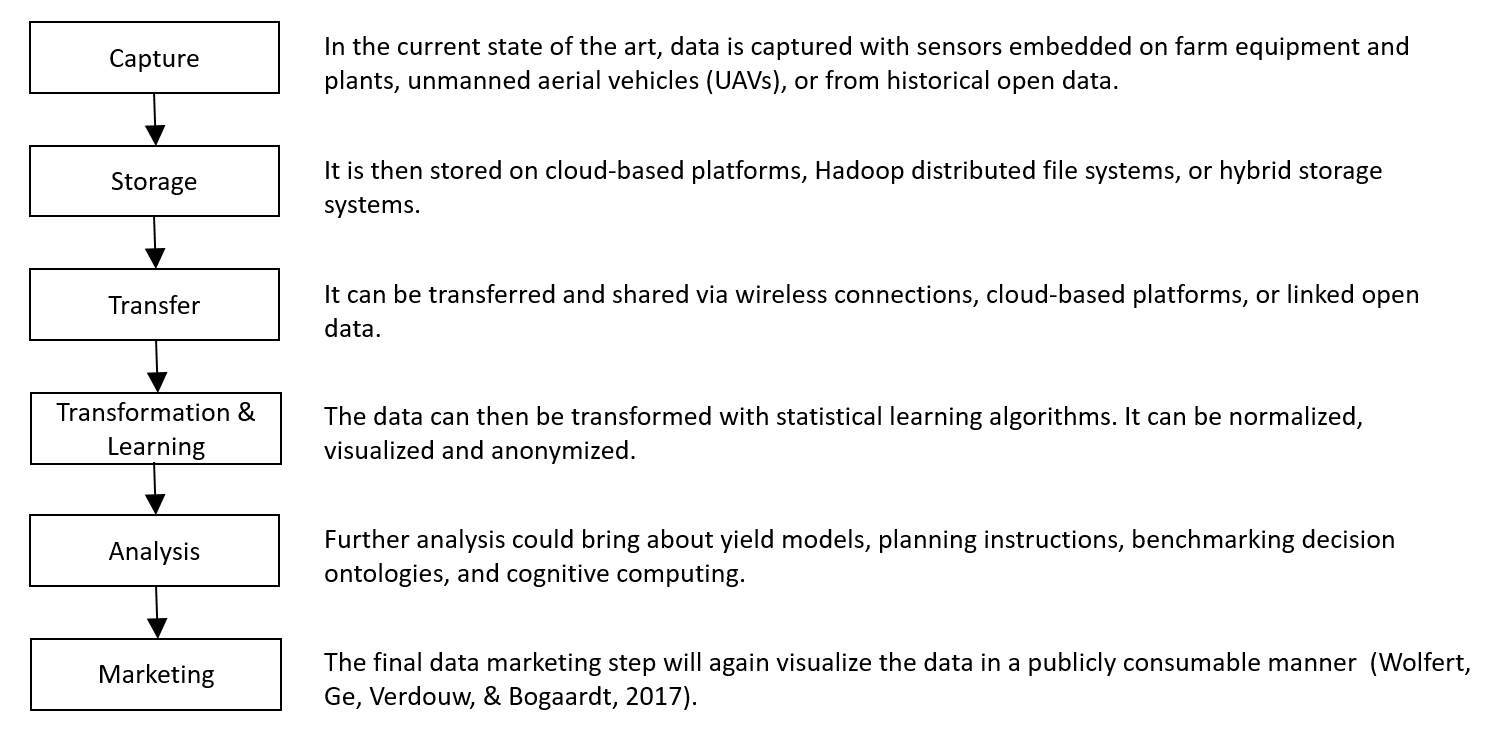
\includegraphics[width=\textwidth,trim={0 0 0 0},clip=true]{Plots/datachain.png}
	\caption{The data chain.} 
	\label{fig:datachain}
\end{figure}

%-------------------------------------
\subsubsection*{Farming Operations}
Ineffective farm operations such as late planting and weeding, the lack of proper land preparation and harvesting techniques, and poor housing and feeding of livestock reduces a farmers� productivity \cite{kshetri2016big}. Big Data can improve performance, and reduce costs in reducing wasted resources (e.g., water and fertilizer). Here, the use of water, fertilizer, and other inputs is likely to involve detailed measurement and monitoring, which can lead to highly personalized (for each farmer) and customized (for each farm) set of solutions. Already, precision agriculture has been a key trend in industrialized countries. 

%-------------------------------------
\subsubsection*{The Land} 
% \shortciteA{sovani1966boserup} proposes three possible strategies for agricultural development: (1) bringing under cultivation of virgin land; (2) \textit{labor-intensive} strategy of cropping more densely, and engaging in more intensive weeding and harvesting; or (3) \textit{capital-intensive} strategy of increasing investments in fertilizer, organic matter, machinery, equipment, and other forms of capital \cite{sovani1966boserup}. The divisions between these strategies for increasing yields are blurry as farmers can decide to implement multiple strategies. 

Some argue that Big Data will shift farming activities towards capital intensiveness and reduce the land degradation problem \cite{kshetri2016big}. However, we can also imagine that much like mechanized equipment and chemical inputs of the past, Big Data, can also be used to allow more frequent cropping of the land, therefore, increasing land degradation. Population growth, specifically more demand for agricultural products, determined whether mechanized equipment and chemical inputs was either labor-saving or land-saving \cite{sovani1966boserup}. The same can be said for Big Data's consequences on farming; the factor influencing agricultural productivity, amount of land under production, and its degradation is demand. That is, Big Data in and of itself will not have a direct impact on lands. 

%-------------------------------------
%\subsubsection*{The Food}  
%Genetically modified food, to finding natural gene combinations. COMPLETE LATER!!!!!

%-------------------------------------
\subsubsection*{Human Labor} 
The human labor behind machine learning is currently happening in two forms: well paid programmers, and low skilled workers. Programmers are currently paid well because of the low supply of those with the required skill sets. Low skilled workers produce the training data sets that get fed into the machines (e.g., farmers agreeing to gauge and report their water use). There are concerns for this second group, which is larger and performs most of the labor, that raises questions about working in this new economy. Currently, the invisible labor of those who either make the training sets or those who are willingly or unwittingly giving up their data, is not paid according to the profits it generates. More data may make our models produce better results, but it�s not clear who benefits and how much. Jaron Lanier, an American computer philosophy writer, has proposed that ordinary people receive ``nano payments" for the big data they generate. Others have proposed recommendations for appropriate guidelines in digital labor rights, but their examination is outside the scope of this paper. 

%-------------------------------------
\subsubsection*{Privacy \& Security}  
Data scraped from farmers unknowingly (e.g., from UAVs and satellites) brings up issues of privacy and consent. While farmers have concerns about data ownership, they also see how much companies are investing in Big Data. To them, the New-England-farmer rule applies here: ``never be the first to try something, nor the last"; that is, farmers want to make sure they reap the profits from Big Data too. Such thinking may lead to new business models that allow for shared harvesting of value from data.

%-------------------------------------
\subsubsection*{Ownership}  
In the current climate, power differences in agribusiness usually come with size differences. The concentration of wealth in just a handful of companies has allowed them to deploy data gathering and statistical learning techniques when a mere couple decades ago that ability was reserved for the governmental agencies operating on pooled tax-based resources. These big agribusiness companies control a massive amount of farming data that may present business risks to small farmers. Furthermore, these large companies exist exclusively in industrialized countries, which have had opportunities to learn from their mistakes and experiences, while farmers based in the developing world have lacked such opportunities \cite{kshetri2016big}. 

Acknowledging these power differences is the first step in changing who owns the data and who shoulders the responsibility of preserving and protecting the data. This responsibility should not be left to corporations because like industrializers of the past, they will engage in information feudalism by deploying intellectual property rights to lock up information from their competitors. Securing a wall of patents that would guarantee monopoly profits, stifles competition and creativity \cite{drahos2017information}. Like feudalism that denied property rights to most of the population (i.e., serfs and slaves) information feudalism will deny small farmers data and its products. Also, like feudalism, information feudalism will reward guilds instead of inventive individual citizens. More importantly, it will eventually rob the knowledge economy of much of its productivity.  

%-------------------------------------
\subsubsection*{Unintended Over Regulation} 
The availability of environmental data can help environmental and land-use agencies introduce and enforce regulation on public resoursces to minimize the excessive use of fertilizers and toxic pesticides \cite{kshetri2016big}. Although such regulation is generally beneficial for the environment, better management of public resources (e.g., land and water) can come at a cost of possibly excessive surveillance, bureaucratization, and a new culture of resources being owned by the state rather than the people. 

One example of a regulatory practice is \textit{The Reasonable and Beneficial Use Doctrine}, the cardinal principle of California water law, which states that all water rights, and all uses of water, must be reasonable. Because of the variable definition of ``reasonable use" the law renders all water rights fragile \cite{gray2015reasonable}. Due to this doctrine, in California water law, there is always an ongoing balance to be struck between the public's welfare and the individual liberties of users. This flexibility also allows for over regulation.

%-----------------------------------------------------------------------------------------------------------------------------------------------------------------------------------------------------
\subsection{Sociological Theory}
Here, we describe agriculture in this new age from multiple angles presented in sociological theory.

%-------------------------------------
\subsubsection*{Dehumanization: Weber and Ritzer} % section 4.1.1 of class
In his research, Weber focused on one type of rationality he called \textit{formal rationality}, a characteristic of bureaucracies in which specialized experts will turn to rules, regulations, and larger social structures to obtain a means-to-an-end, and virtually everyone will take the same optimal path to achieve a goal (\citeNP{weber2013max}; \citeNP{ritzer2004mcdonaldization}). This concept is also seen to varying degrees in artificial intelligence, machine learning, and data-driven decision making, which attempt to replace human judgement with rational rules. One such algorithm is even called a rules-based-expert system. In such systems, rationality is developed on how we have behaved in the past. After all, all machine learning models learn a behavior, a tendency, and a personality from past data, and then predicts that thing they've learned with cold accuracy \cite{foreman2014humanity}. Furthermore, by letting predictions made on past data influence our decision making, we are bringing the past into the present. Therefore, these models also act as echo chambers, reinforcing past truths.

Weber described bureaucracy as rational systems concerned with the efficient attainment of an organization's goals. Weber's ``ideal" bureaucracy has written rules of conduct, specialized divisions of labor and is hierarchical, impersonal, and efficient. Therefore, a bureaucracy's dehumanization is meant for efficiency. However, in practice, bureaucracies are infamous for their inefficiency and irrationality, because there will always be elements in a process which escape calculation. That is, until all human intelligence can be modeled, there will always be elements of cognition which cannot be replicated by a machine. Therefore, like in bureaucracies, human intervention is sometimes necessary. 

%-------------------------------------
\subsubsection*{Scientific Management: Taylor} % section 4.2.2 of class
According to \shortciteA{taylor1914principles}, the worker most suited to handling the actual work is unable to understand the real science of doing this class of work! Instead, enlightened specialists should govern the labor process according to scientific principles, and this is to be rendered independent of craft, tradition, and the workers knowledge \cite{taylor1914principles}. This divorce of conception from execution leads to the dehumanization of the labor process, and ``the administration of things" is to exterminate inefficiencies. 

``Efficiency" in this rational system will come at a cost to the workers; workers will lose control over their own labor and manner of its performance. Also, as the science of the labor process grows it will no longer be in the hands of the workers, but will be concentrated in the hands of management. Such hierarchy negates the value of the worker's practical and experiential knowledge, since those aspects of the labor process may not be captured in data available to management. % example of vernacular agriculture.  

``Scientific" agriculture brings similar concerns over who owns the data, the science of the means of agricultural production, and the control over operations and labor. It is likely that farmers will lose control over the vastly unappreciated control of the workday, of when to plant, how to cultivate, when to harvest and sell, and so forth. Farm labor will change to be much more like in the days of automation, when autonomy and independence became tied to the clock, the rhythm of the machine, and closely monitored. 

So far, scientific agriculture has favored regimented agricultural practices which is large, capital-intensive, and single crop (often a hybrid or clone for maximum crop uniformity). Under such systems, crops are grown in straight rows for easy tillage and machine harvesting, and fertilizers, irrigation, pesticides, and herbicides are used to make fields suitable \cite{scott2012two}. \shortciteA{scott2012two} calls this regularity the cult of geometry. The effort of this agriculture is to rise above, as it were, local soils, landscapes, labor, implements, and weather. The antithesis to this ``pageantry" of symbolic order is \textit{vernacular agriculture} where farmers poly crop, plant crops that are finely tuned to local conditions, and the fields often have visual disorder. Surprisingly, visual disorder does not immediately equate to inefficiency, as visual order is not necessarily equal to working order either \cite{scott2012two}. In the same vein as vernacular agriculture, \textit{conservation agriculture} attempts to have minimal land disturbances (e.g., with plows and tractors), constant land cover (i.e., with cover crops), and crop rotation and intercropping \cite{hobbs2007conservation, giller2015beyond}. This form of farming promises the sustainability of agriculture since through its practice land is preserved and not degraded for future generations \cite{hobbs2008role}. 

Lastly, the dehumanized system that emerges from scientific agriculture, creates a hierarchical and authoritarian climate where workers will learn habits of deference. Jean-Jacques Rousseau believed that such settings created the personalities of subjects rather than citizens; subjects learned the habits of deference. In extreme cases, \textit{institutional neurosis} sets in, where people lack interest in their surroundings, make no plans, lack spontaneity \cite{scott2012two}, and eventually may experience the death of independent opinion, let alone a controversial one.

% ``The scientific community, while excluding the public will claim to play no favorites, take no discretionary action, have no biases, merely making transparent technical calculations. The criteria for decisions are explicit, standardized and known in advance. Discretion and politics are made to disappear by techniques that are at bottom completely saturated with discretionary choices and political assumptions, now shielded effectively from public view. " \cite{scott2012two}...... consequences, class separations.

%-------------------------------------
\subsubsection*{The Growth Trap: Rushkoff}
Agriculture began in at least eight different parts of the world (e.g., equatorial regions, South America, and Papua New Guinea; \citeNP{larson2014current}; \citeNP{vavilov1992origin}). Although there are controversies surrounding the speed, intentionality, and evolutionary aspects of the domestication process, all regions are becoming progressively efficient in agricultural production and are following the same developmental steps (for these steps see Appendix \ref{g:history}). This progressive movement towards efficiency embodies ``the growth trap". \shortciteA{rushkoff2016throwing} explains the growth trap as an imperative process for corporations. Unlike natural organisms that can reach a level of maturity where health is no longer about growing but about maintaining, corporations are duty bound to grow by any means necessary \cite{rushkoff2016throwing} and therefore, never reach equilibrium. The same efficiency requirements govern growth in agriculture. 

The growth trap is not one we have most recently walked into; the growth trap is and has been more a feature of our world and the agricultural system, than a bug. Therefore, it would be difficult for society to divest from the desire to be efficient; we cannot escape the disruptive impact of the digital economy and its inevitable structural break down as we run out of places to extract value for growth. One consequences of this feature is that decisions are made to satisfy criteria which are purely economic.

%-----------------------------------------------------------------------------------------------------------------------------------------------------------------------------------------------------
\subsection{Recommendations} 
According ing to \shortciteA{frase2016four} two of society's biggest threats are the scarcity and abundance of natural resources: scarcity that is inevitable with climate change, and abundance that is to come from artificial intelligence. Although, it may sound contradictory, we are currently facing this dual crisis through the rapid spread of computerization in our economy, including the traditional sectors of agriculture and manufacturing. 

As we muddle through the problems that are coming from climate change and artificial intelligence, we should resist falling into the crude techno-utopian versus techno-skeptic dichotomy, because these struggles with technology are never just about the technology itself; they are ultimately about the balance of class power \cite{frase2015ours}. The Luddites, for example, were portrayed as hostile to weaving machinery, which had manifestly positive qualities (i.e., more efficient generation of wealth), and therefore, were dismissed as selfish or irrational (because who can rationally argue against more wealth). However, their sabotage (i.e., breaking of machines) was not due to the textile workers directing their anger at the technology per se, but, as a means to coerce their employers into granting them concessions. To the capitalist, there is no difference between machine sabotage and other kinds of labor action, since in both cases, value is destroyed; all worker resistance is Luddism \cite{frase2015ours}. Understanding this, workers would revolt. Today, technology continues to exasperate the imbalances in class. To defend against it, in the agricultural industry we can assert the purpose of economic growth, re-examine what we mean by intelligence, and realize the value of diversity in crops.  

%-------------------------------------
\subsubsection*{Purpose of Economic Growth}
We need to assert the purpose economic growth; that is, we need to clearly demarcate who benefits and how much. As it stands, we have two choices: the possibility of a better life with less labor (and more leisure time to be creative/innovative) or to face mass unemployment (and continued wealth and income inequality). Some  have proposed solutions, such as universal basic income, federal jobs guarantee, or public works as a means to redistribute wealth, but the examination of their merits are outside the scope of this paper.  

%-------------------------------------
\subsubsection*{Meaning of Intelligence}
We need to re-examine what we mean by ``intelligence." In our current system, only the formal ways in which a computer can use data is considered intelligent; we consider the forms of intelligence that can be coded for a computer (e.g., numerical data) to be valuable. Naturally, in such a system, we will collect, preserve, and curate this form of data until all others are lost. 

\shortciteA{whyte2017indigenous} explains that scientists often appreciate what he calls the supplemental-value of indigenous knowledges, which is the value of Indigenous knowledges as inputs for adding (i.e. supplementing) data that scientific methods do not normally track. However, farmers have produced and consumed many different forms of data. Traditional Ecological Knowledge is part science, part practice, and part belief system \cite{reo2012hunting}. All three spheres of knowledge contribute to, for example, the hunting practices of North American Native Tribes and their adaptation to climate change. Should we not also appreciate the governance-value of the knowledge these tribes impart, the more informal parts may be lost.

%-------------------------------------
\subsubsection*{Crop Diversity} 
We need to realize the value of diversity in crops. Crop diversity is defined as a high number of crop species, and genetic diversity within each crop type. So far, profits have been a big driver of decision making in California agriculture. This has produced hardening water demand as farmers are turning to more valuable perennial crops (e.g., trees that are a major investment and need constant watering; \citeNP{robthesis}). The transition to perennials is especially risky given the realities of climate change and more weather extremes (i.e., more floods and droughts) and less reliable water supplies (\citeNP{mazur2009indicators}; \citeNP{wuebbles2014cmip5}). Agricultural organization when picking crop types must satisfy criteria which are not purely economic to account for factors such as climate change. 

In addition, with crop type changes, we are forcing our environments into states that are not natural, degradable, and not sustainable; ecosystems only function as self-regulating when they have sufficient biodiversity of plants and animals; a mono-cultured field is highly susceptible to invasive species and less resilient to disease (e.g., the Irish Potato Famine). 

Crop diversity helps with the issue of weakened sovereignty, the disappearing rights of those who produce and consume food to define their own food systems. The expansion of the big seed companies (e.g., Monsanto) is making commercial seeds more common, while intellectual property laws are protecting the companies� patents. This means farmers are losing the right to breed new varieties or even retain their seeds \cite{chun2014decline}. 

Lastly, there is an educational value in having diverse crops available for scientific study. Studying at two agricultural schools myself, I have seen first hand the importance of the availability and ease of access for scientific research that will otherwise not happen. 

%-----------------------------------------------------------------------------------------------------------------------------------------------------------------------------------------------------
\subsection{Conclusion}
We are sufficiently far from a time when humans are completely superfluous to the farming process. Despite our inability to shed off the desire for efficiency, and therefore the chase for bigger better algorithms, we can reward expert-plus empirical systems. Human experts may need to perform tasks involving problems and processes for which no algorithm exists or the algorithm has not yet been developed. For example, in some situations, tasks involving unknown soil types and extreme weather conditions often need to be performed by humans rather than algorithms \cite{kshetri2016big}. Furthermore, algorithms may miss important aspects of farming practices as they are not adept at handling situations that have escaped calculation. 

Currently, neither data-driven models nor the expert relying solely on intuition will do better than a combination of the two \cite{kuhn2013applied}. Humans usually make better predictions when they are provided with the results of statistical prediction; predictive modeling should not be regarded as a substitute for intuition, but as a complement \cite{ayres2007super}. Therefore, our intuition, until it is winnowed down to an algorithm, is still valuable. For such intuition to survive, as a society, we will have to restructure our economic systems, preserve all forms of intelligence, and hold crop diversity just as valuable as pure short term economic gains. 


